\def\layersepp{2.5cm}
\def\layerseppp{5cm}
\def\layersepppp{7.5cm}
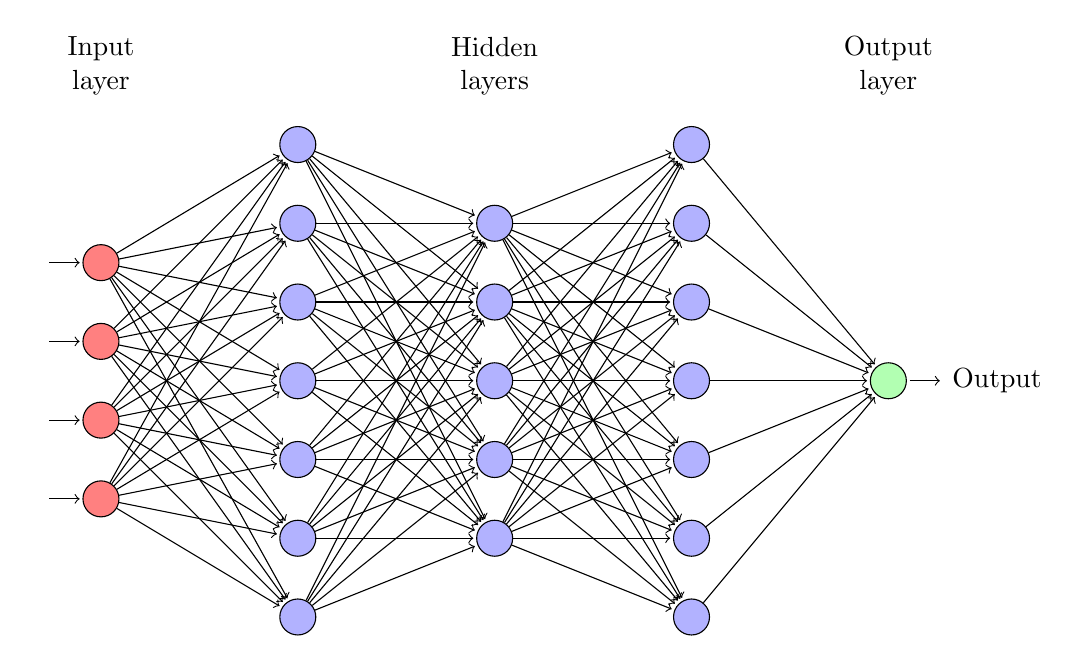
\begin{tikzpicture}[shorten >=1pt,->,draw=black, node distance=\layersepp]
    \tikzstyle{every pin edge}=[<-,shorten <=1pt]
    \tikzstyle{neuron}=[circle, draw,minimum size=13pt]
    \tikzstyle{input neuron}=[neuron, fill=red!50];
    \tikzstyle{output neuron}=[neuron, fill=green!30];
    \tikzstyle{hidden neuron}=[neuron, fill=blue!30];
    \tikzstyle{annot} = [text width=4em, text centered]

    % Draw the input layer nodes
    \foreach \name / \y in {2,...,5}
    % This is the same as writing \foreach \name / \y in {1/1,2/2,3/3,4/4}
        \node[input neuron, pin=left:] (I-\name) at (0,-\y) {};

    % Draw the hidden1 layer nodes
    \foreach \name / \y in {1,...,7}
        \path[yshift=0.5cm]
            node[hidden neuron] (H1-\name) at (\layersepp,-\y cm) {};

    % Draw the hidden2 layer nodes
    \foreach \name / \y in {2,...,6}
        \path[yshift=0.5cm]
            node[hidden neuron] (H2-\name) at (\layerseppp,-\y cm) {};

    % Draw the hidden3 layer nodes
    \foreach \name / \y in {1,...,7}
        \path[yshift=0.5cm]
            node[hidden neuron] (H3-\name) at (\layersepppp,-\y cm) {};

    % Draw the output layer node
    \node[draw, output neuron,pin={[pin edge={->}]right:Output}, right of=H3-4] (O) {};

    % Connect every node in the input layer with every node in the
    % hidden layer.
    \foreach \source in {2,...,5}
        \foreach \dest in {1,...,7}
            \path (I-\source) edge (H1-\dest);

    \foreach \source in {1,...,7}
        \foreach \dest in {2,...,6}
            \path (H1-\source) edge (H2-\dest);

    \foreach \source in {2,...,6}
        \foreach \dest in {1,...,7}
            \path (H2-\source) edge (H3-\dest);

    % Connect every node in the hidden layer with the output layer
    \foreach \source in {1,...,7}
        \path (H3-\source) edge (O);

    % Annotate the layers
    \node[annot,above of=H2-2, node distance=2cm] (t1) {Hidden layers};
    \node[annot,left of=t1, node distance=5cm] {Input layer};
    \node[annot,right of=t1, node distance=5cm]{Output layer};
\end{tikzpicture}
